%!TEX root = dissertation.tex
%%%%%%%%%%%%%%%%%%%%%%%%%%%%%%%%%%%%%%%%%%%%%%%%%%%%%%%%%%%%%%%%%%%%%%%%%%%%%%%%
%
% Collection of all relevant mobile radio specifications and descriptions
%
\section{Übersicht}

\begin{itemize}
\item Einarbeitung
	\begin{itemize}
		\item Architektur von 3G-Netzen
		\item Modelle zur Beschreibung von Datenverkehrsflüssen
		\item Einarbeitung in das Messsystem des FTW
	\end{itemize}
\item Definition eines einfachen Bearer-Modells
\item Programmierung der Auswertung
\item Durchführung und Auswertung der Messungen
\item Anfertigung eines Berichtes
\end{itemize}

\section{Modeling}
Macroscopic Behavior

	-- time Connection Setup until Call Termination with Talk Spurts
	--> ON/OFF Process
	--> Empricial measurement
	
Source Traffic Model
	-- 2 parts: 
		arrival process for user activities
		process describing activity phase
	-- arrival time:
		User begins web browsing
	
Simulation \& Software
	ns-2 UMTS mobile parts only
	ns-3 GSoC2010 implementing \ac{UTRAN} (MAC\&PHY) incl radio bearers (+OpenFlow)
	Harald Welte GPRS: OpenBSC, OpenGGSN incl GTP
	

EPS first introduced in 3GPP Release 8, completed in March 2009. Consisting of EUTRAN, EPC (formerly SAE)


	


\begin{figure}[htbp]
 \centering
 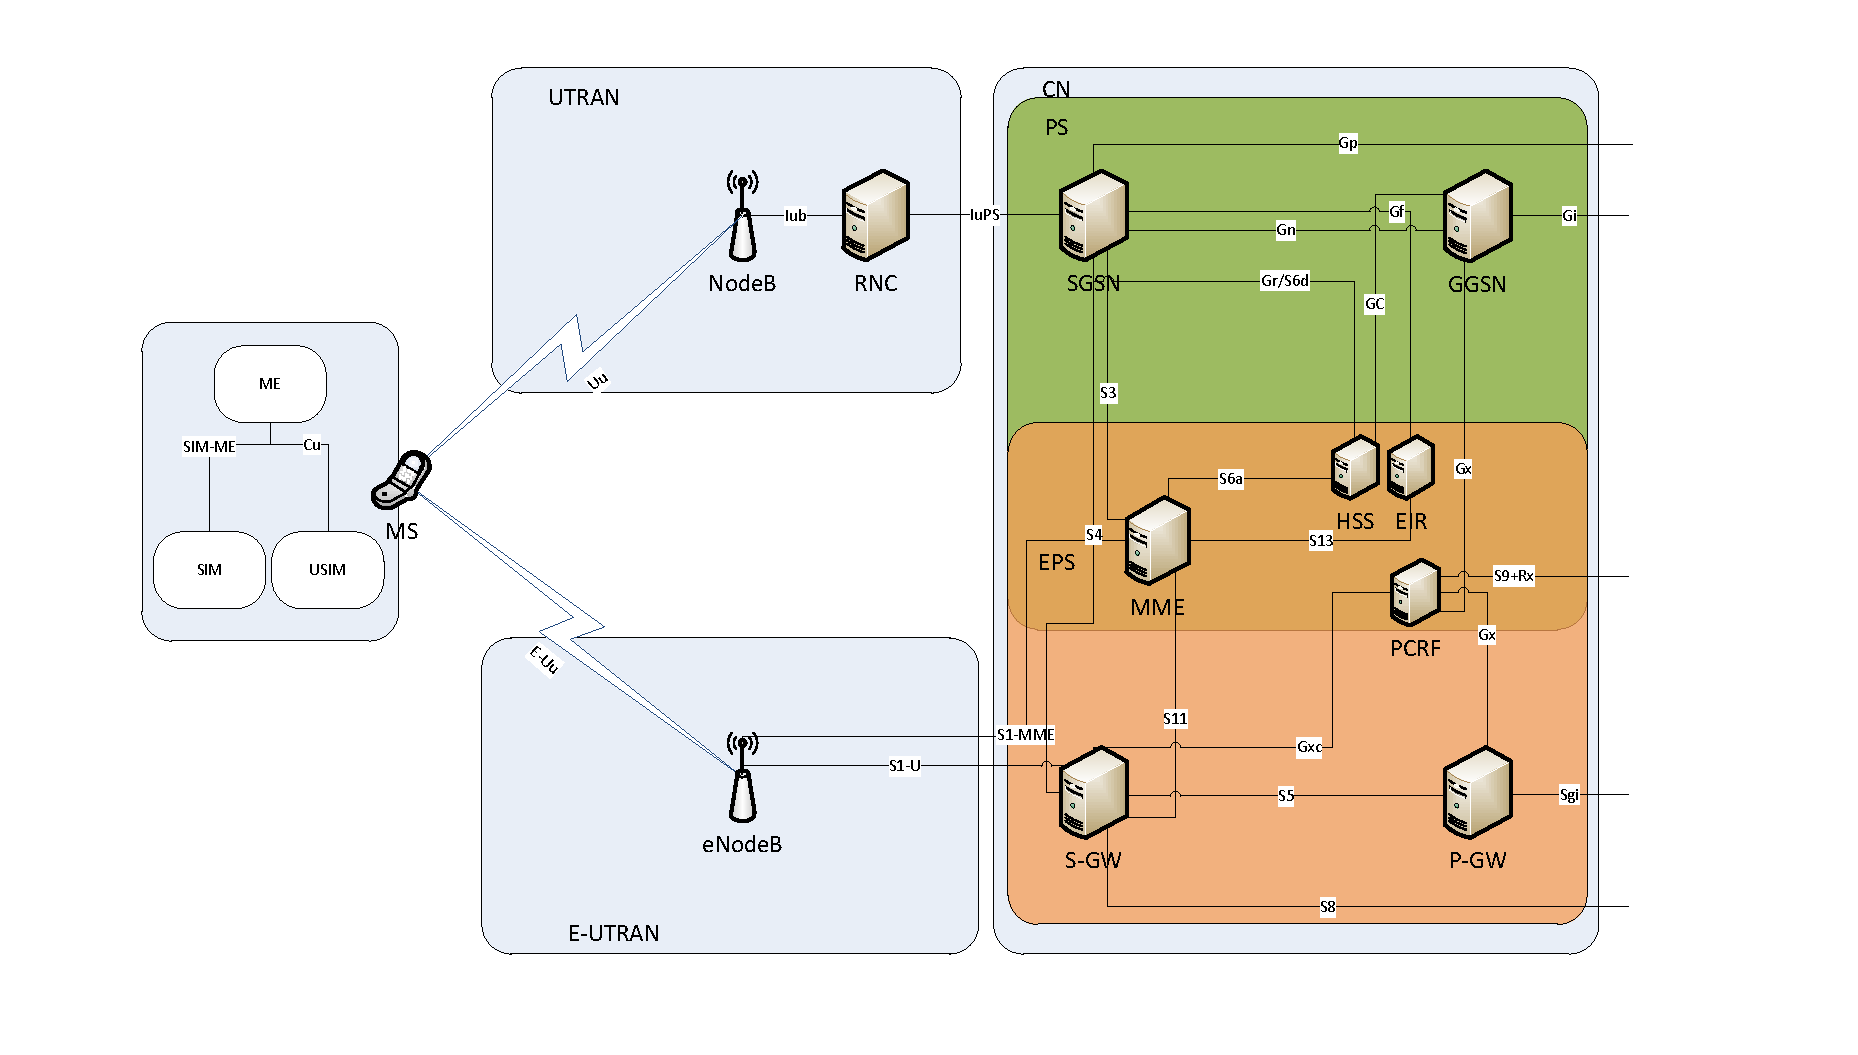
\includegraphics[width=1.0\textwidth]{images/3gpp/eps_ps-overview.pdf}
 \caption{Beispielnetz}\label{fig:netzwerk2}
\end{figure}

List of interfaces in the 3G/LTE PS network
\begin{itemize}
\item \textbf{Uu}: Interface between the mobile station (MS) and the fixed network part in Iu mode. The Uu interface is the Iu mode network interface for providing packet data services over the radio to the MS. The MT part of the MS is used to access the UMTS services through this interface.
\item \textbf{Iub}: Interface between a NodeB and a RNC.
\item \textbf{IuPS}: Interface between a RNC and a SGSN.

\item \textbf{S1-U}: Interface between a eNodeB and a S-GW. User plane bearer tunneling.
\item \textbf{S1-MME}: Interface between a eNodeB and a MME.
\item \textbf{S3}: Interface between a SGSN and a MME. User/bearer information exchange for active/idle state 3g network access mobility.
\item \textbf{S4}: Interface between a SGSN and a S-GW.	 2G user plane tunneling. GPRS mobility and control.
\item \textbf{S5}: Interface between a S-GW and a P-GW within the same PLMN. User plane tunneling; S-GW relocation due to mobility.
\item \textbf{S6a}: Interface between a MME and a HSS. Auth/auth data transfer to evolved system.
\item \textbf{Gr/S6d}: Interface between a SGSN and a HSS. 
\item \textbf{S8}: Interface between a S-GW and a P-GW in different PLMNs. Inter-PLMN variant to S5.
\item \textbf{S9}: Interface between a PRCF and the packet data network. Data exchange to visited PCRF PLMN.
\item \textbf{S11}: Interface between a S-GW and a MME.
\item \textbf{S12}: UTRAN to S-GW reference point. Based on Iu-u/Gn-u. Direct Tunnel via GTP-U.
\item \textbf{S13}: Interface between a MME and a EIR. UE identity check.
\item \textbf{SGi}: The reference point between the EPC based PLMN and the packet data network. Same as Gi for 3gpp.

\item \textbf{GC}: Interface between a HSS and a GGSN.
\item \textbf{Gf}: Interface between a SGSN and a EIR.
\item \textbf{Gi}: Reference point between Packet Domain and an external packet data network.
\item \textbf{Gn}: Interface between two GSNs within the same PLMN.
\item \textbf{Gp}: Interface between two GSNs in different PLMNs. The Gp interface allows support of Packet Domain network services across areas served by the co-operating PLMNs.
\item \textbf{Gx}: Interface between a PCRF and a P-GW/GGSN. QoS policy and charging rules transfer.
\item \textbf{Gxc}: Interface between a PCRF and a S-GW.

\item \textbf{Rx}: Interface between a PRCF and the packet data network.
\end{itemize}

\section{Control Plane Protocol Stacks}

\begin{figure}[htbp]
 \centering
 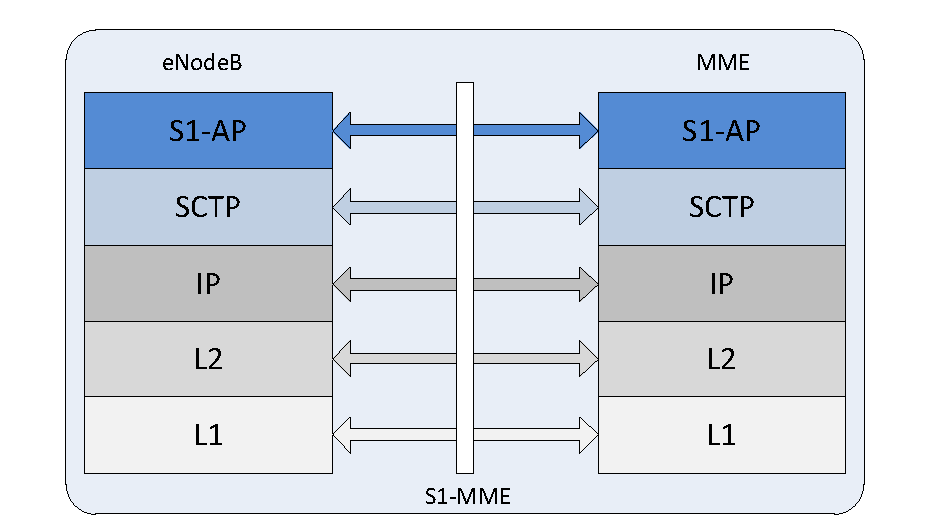
\includegraphics[width=1.0\textwidth]{images/3gpp/eNB-MME-layers.pdf}
 \caption{Beispielnetz}\label{fig:3gpp-enbmme}
\end{figure}

\begin{figure}[htbp]
 \centering
 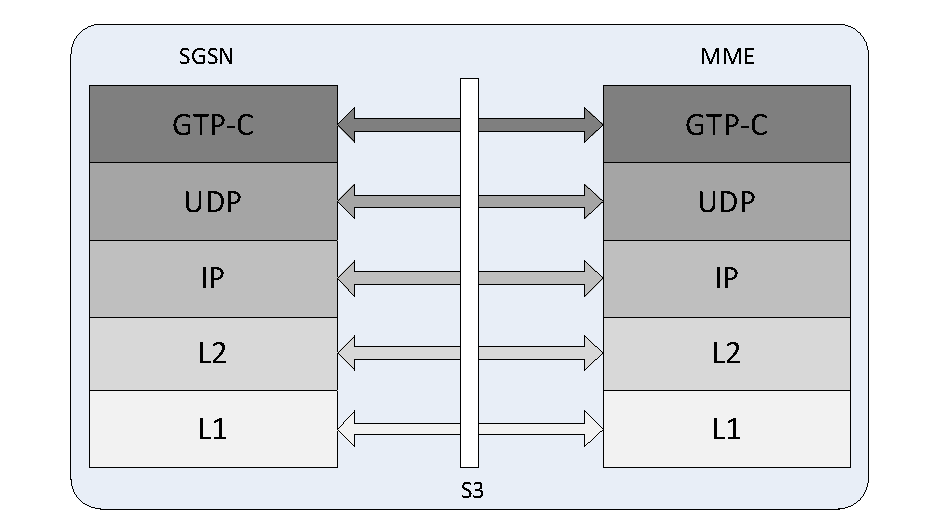
\includegraphics[width=1.0\textwidth]{images/3gpp/SGSN-MME-layers.pdf}
 \caption{Beispielnetz}\label{fig:3gpp-sgsnmme}
\end{figure}

\begin{figure}[htbp]
 \centering
 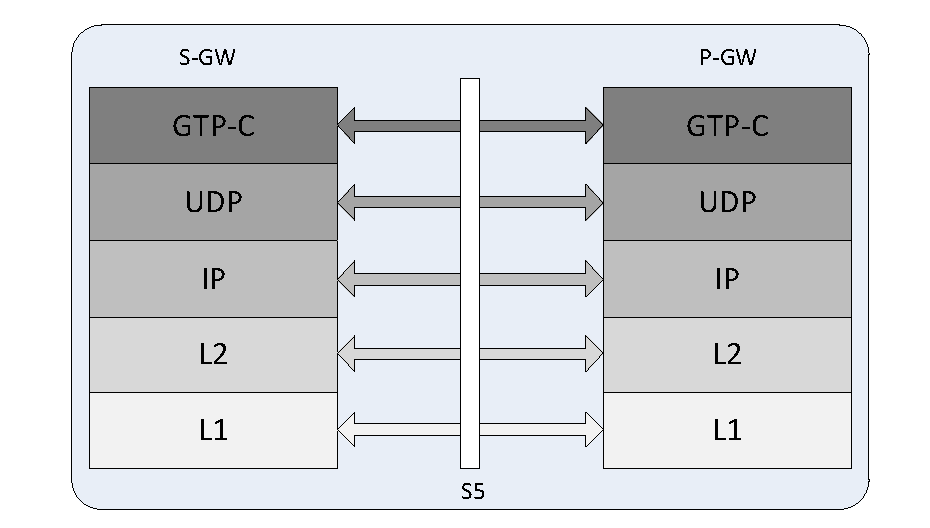
\includegraphics[width=1.0\textwidth]{images/3gpp/S-GW-P-GW-layers.pdf}
 \caption{Beispielnetz}\label{fig:3gpp-sgwpgw}
\end{figure}

\begin{figure}[htbp]
 \centering
 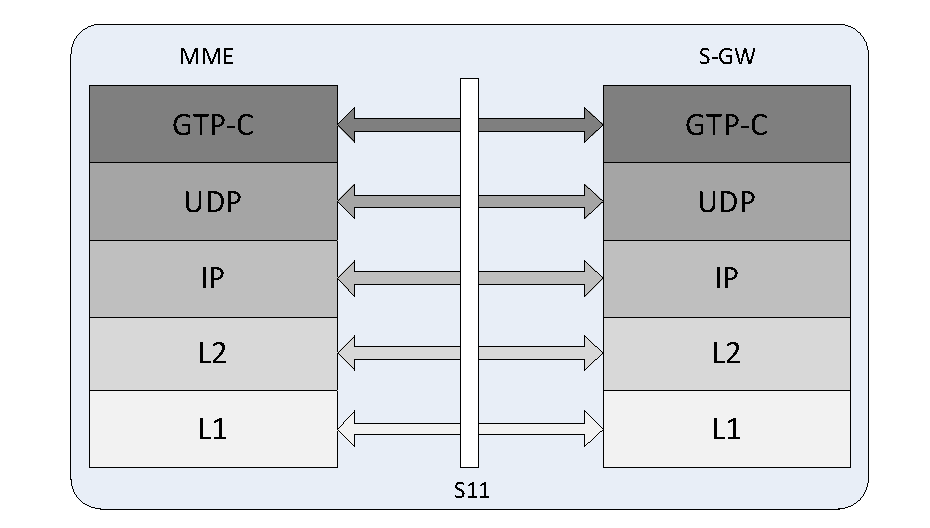
\includegraphics[width=1.0\textwidth]{images/3gpp/MME-S-GW-layers.pdf}
 \caption{Beispielnetz}\label{fig:3gpp-mmesgw}
\end{figure}


\begin{figure}[htbp]
 \centering
 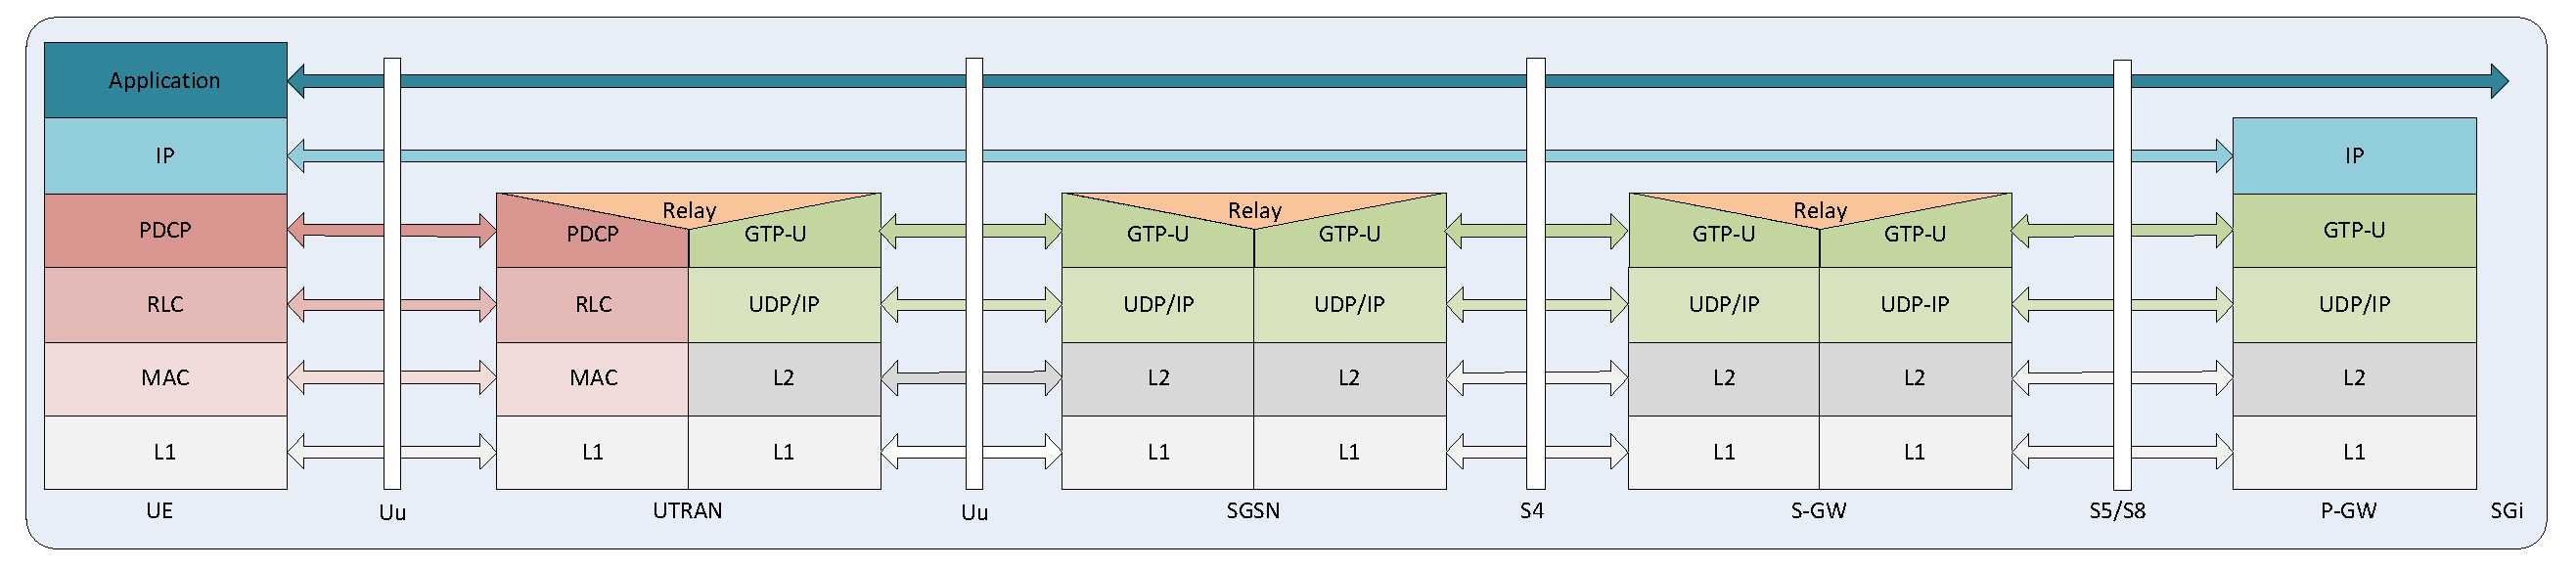
\includegraphics[width=1.0\textwidth]{images/3gpp/3g-userplane.pdf}
 \caption{Beispielnetz}\label{fig:3gpp-umtsuserplane}
\end{figure}

\begin{figure}[htbp]
 \centering
 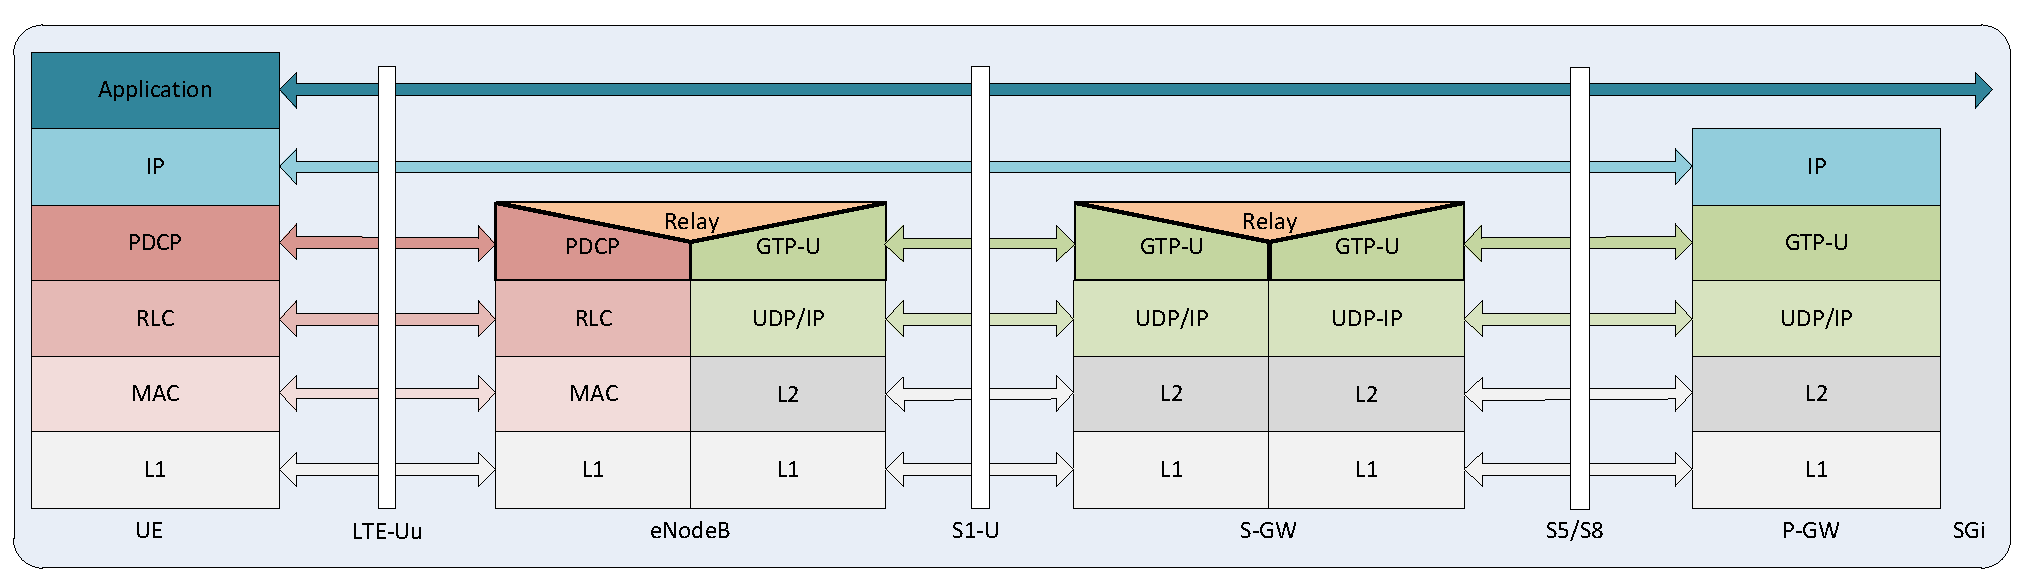
\includegraphics[width=1.0\textwidth]{images/3gpp/LTE-userplane.pdf}
 \caption{Beispielnetz}\label{fig:3gpp-lteuserplane}
\end{figure}


\section{Bearers}

As you said only 11 bearer are permitted.
So PDN connection(Default bearer) + Dedicated bearers put together should not exceed 11 bearers at any instant of time at UE side.
Theoretically 11 PDN connections are possible. But i dont think it will be of any use in practical EPS topology.

One UE Can have Maximum 3 PDN connection.
where as my knowledge is concern one UE can support maximum 11 bearers, 3 default and 8 dedicated bearers.

Does I will get in any spec for this. As the default bearer are of  NON-GBR type and and there are 5-9 are of NON-GBR QCI so I think a ue can have maximum 5 default bearer If two default bearer can not use same QCI.

\begin{figure}[htbp]
 \centering
 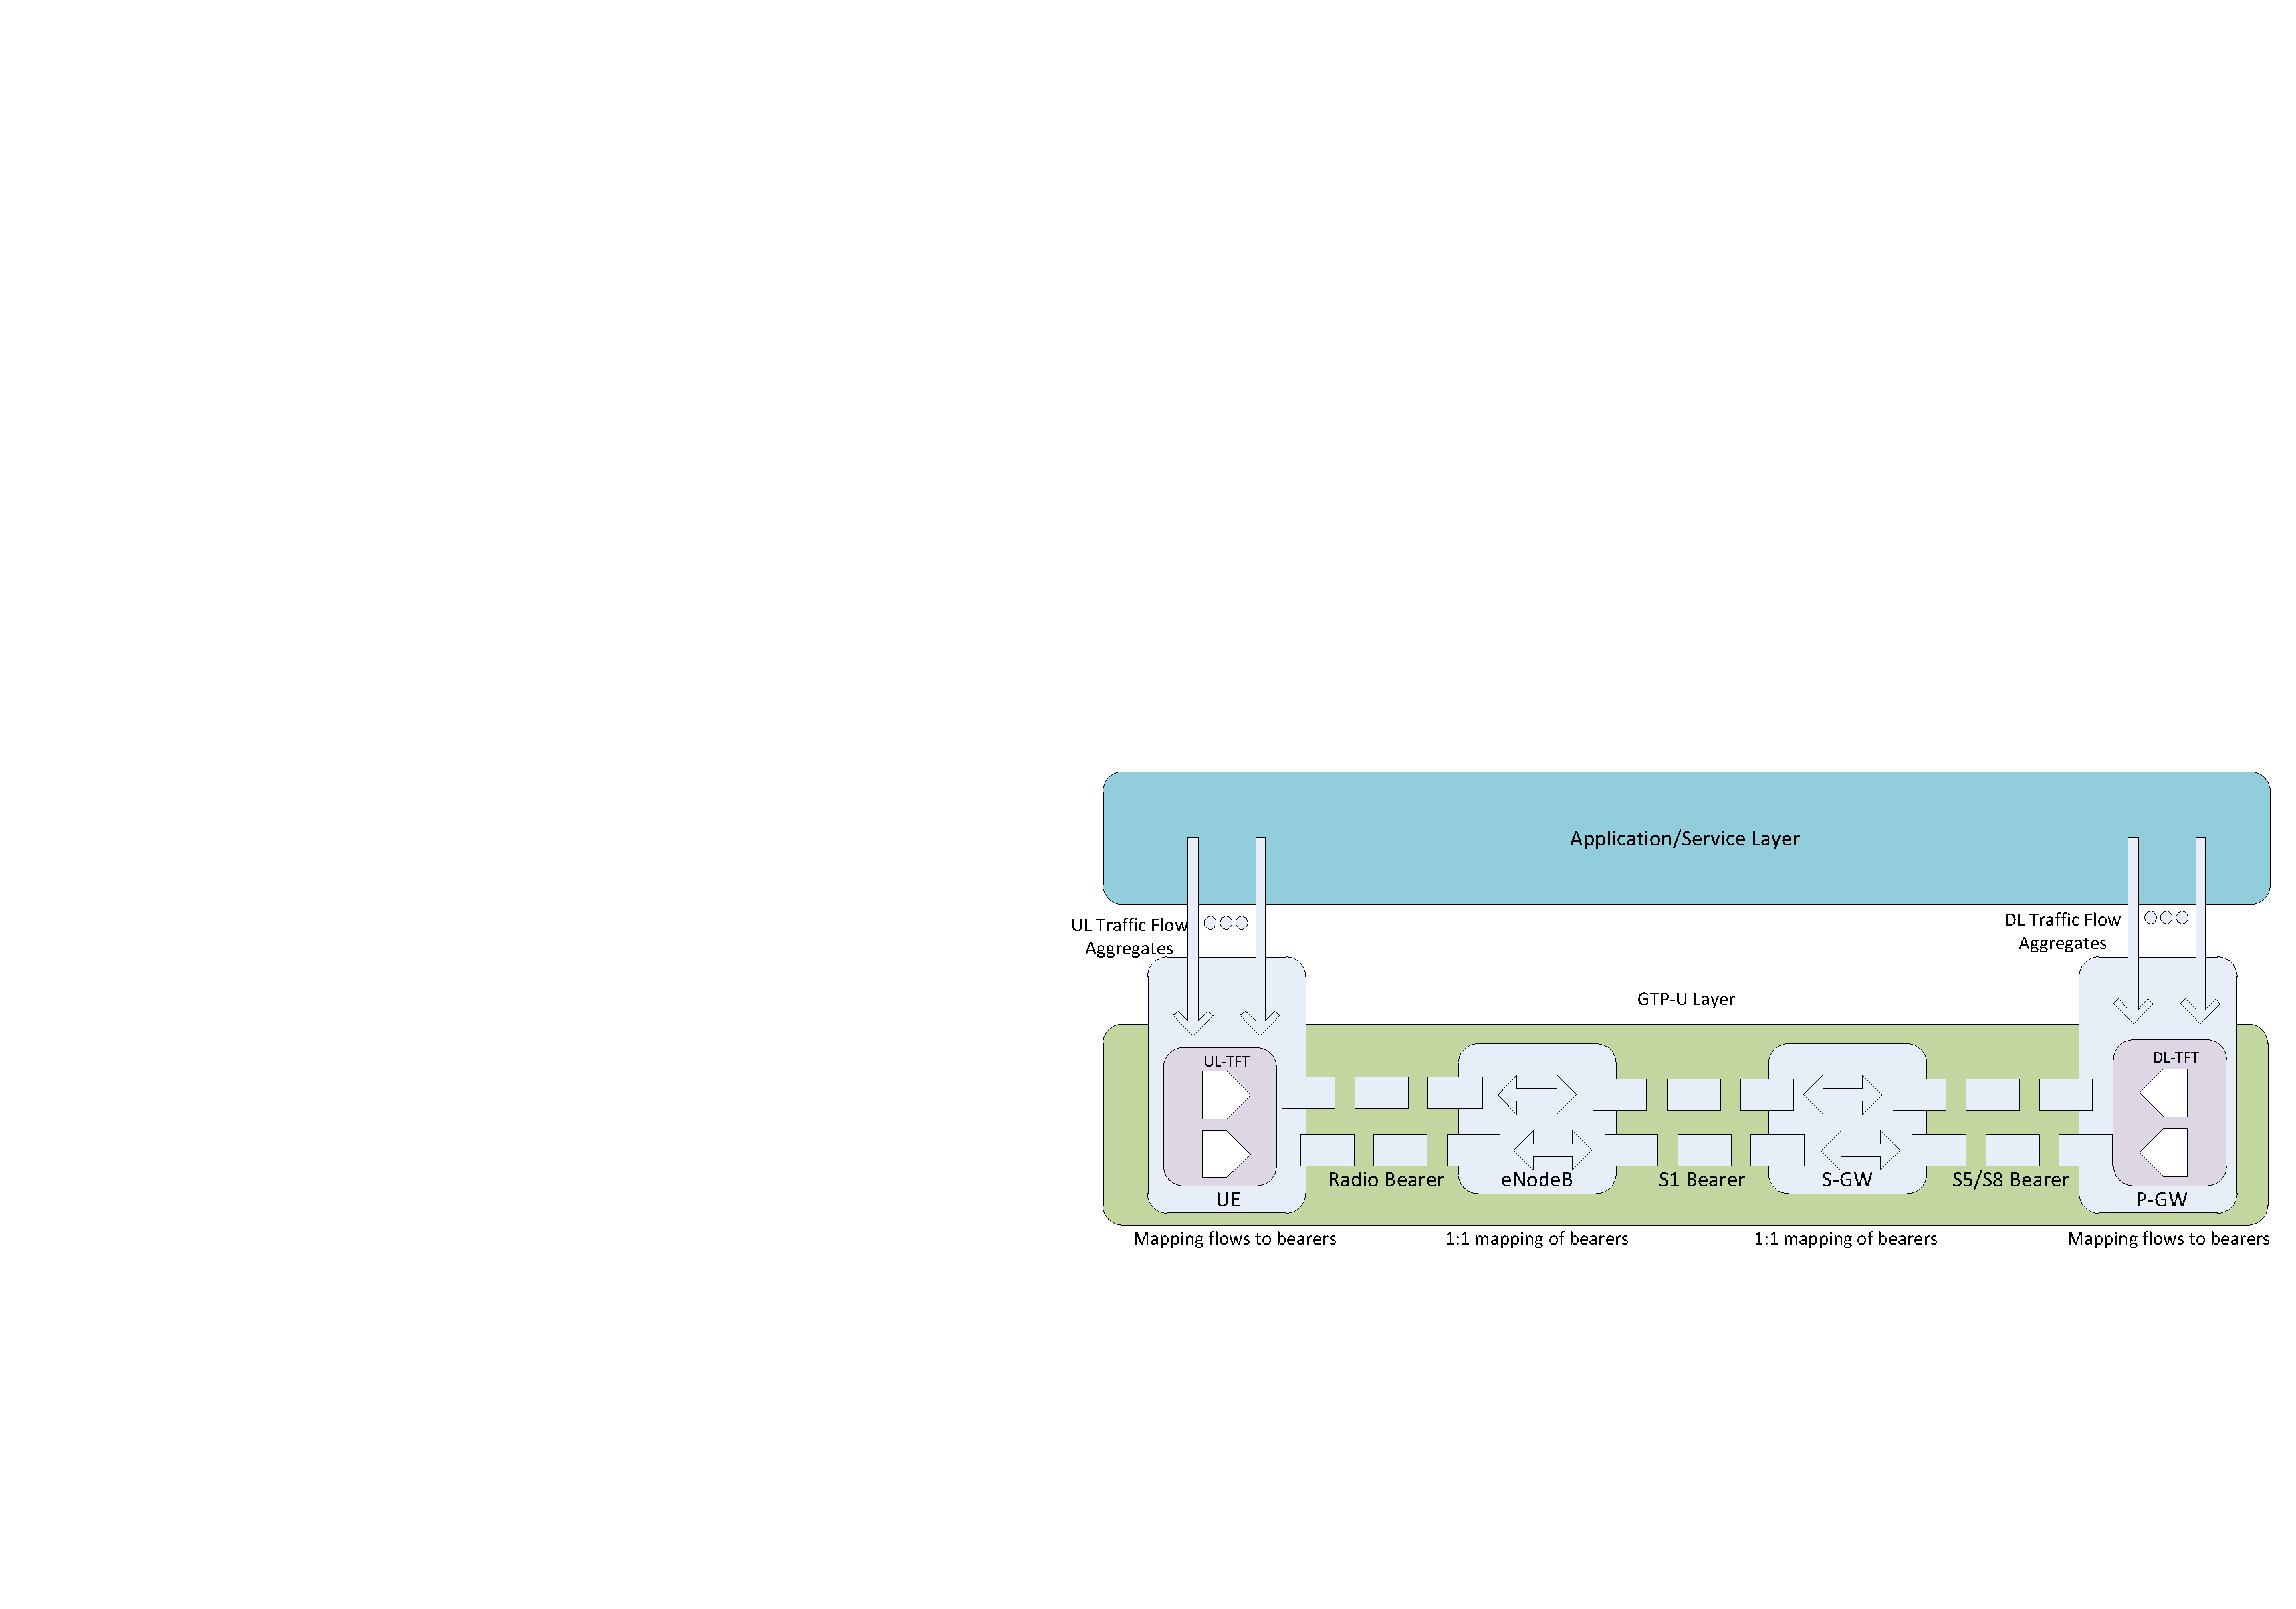
\includegraphics[width=1.0\textwidth]{images/3gpp/bearers.pdf}
 \caption{Beispielnetz}\label{fig:3gpp-bearers}
\end{figure}


\begin{figure}[htbp]
 \centering
 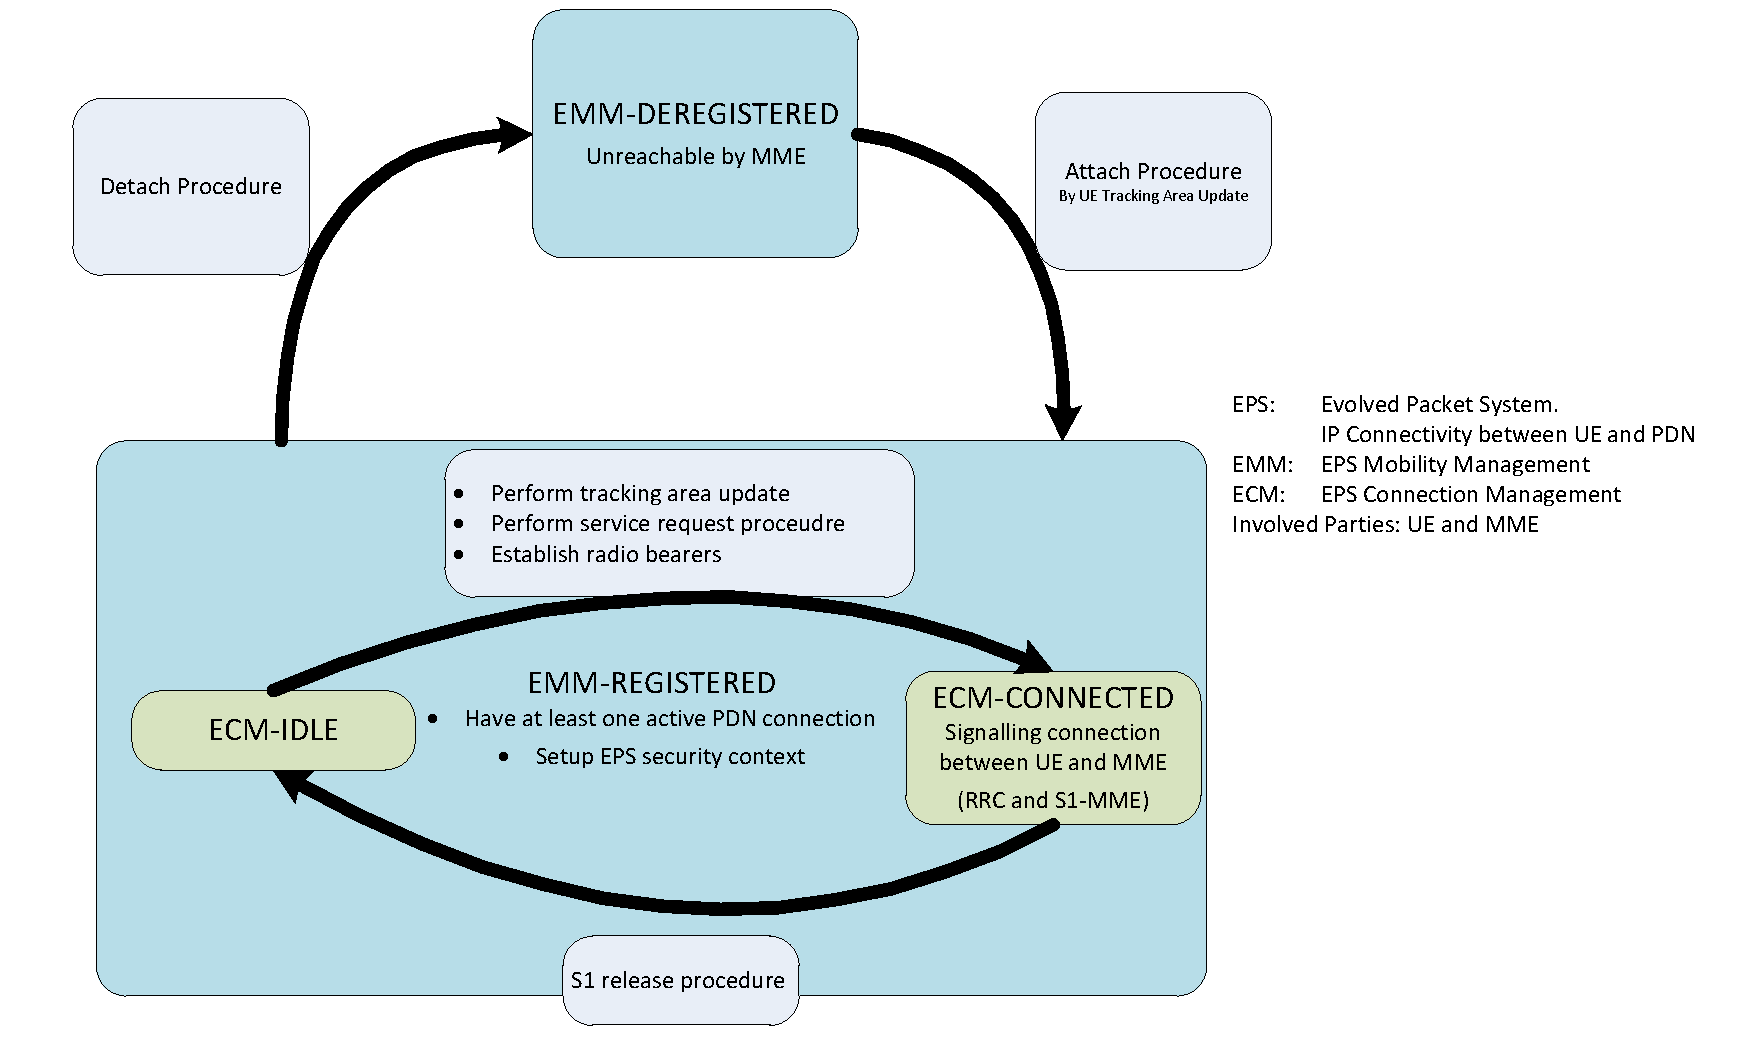
\includegraphics[width=1.0\textwidth]{images/3gpp/ECM-states.pdf}
 \caption{Beispielnetz}\label{fig:3gpp-ecmstates}
\end{figure}

\begin{itemize}
\item 	Every bearer has a predefined QoS level between UE and P-GW.
		==> Level of Granularity for QoS control.
\item	Initial bearer QoS level assigned by network based on subscription data.
\item	Guaranteed Bit Rate (GBR) bearers: dedicated network resources permanently allocated at est/mod. Otherwise Non-GBR.
\item	The Traffic Flow Template (TFT) belonging to a bearer is a set of packet filters that assign traffic flows to the bearer.
\item	UL-TFT at UE, DL-TFT at PCEF (P-GW).
\item 	default bearer: always-on IP connectivity for the UE to a PDN
\item	dedicated bearer:   
			\begin{itemize}
				\item any additional bearer for the same PDN
				\item Traffic Flow Template (TFT) associated with every ded. bearer
				\item establishment/modification decision only by EPC
				\item QoS level assignment only by EPC
			\end{itemize}

\item	default bearer may be used as {m,c}atch-all traffic bearer for everything that does not match any filter
\item	Every bearer associated with QCI and ARP.

QoS class identifier (QCI): standardized scalar as reference for node-specific QoS parameters
Allocation and Retention Policy (ARP): priority level preemption capability, preemption vulnerability.

\item	All simultaneously active bearers by one UE are provided are provided by the same P-GW.
\end{itemize}

EMM Service request procedure

\begin{figure}[htbp]
 \centering
 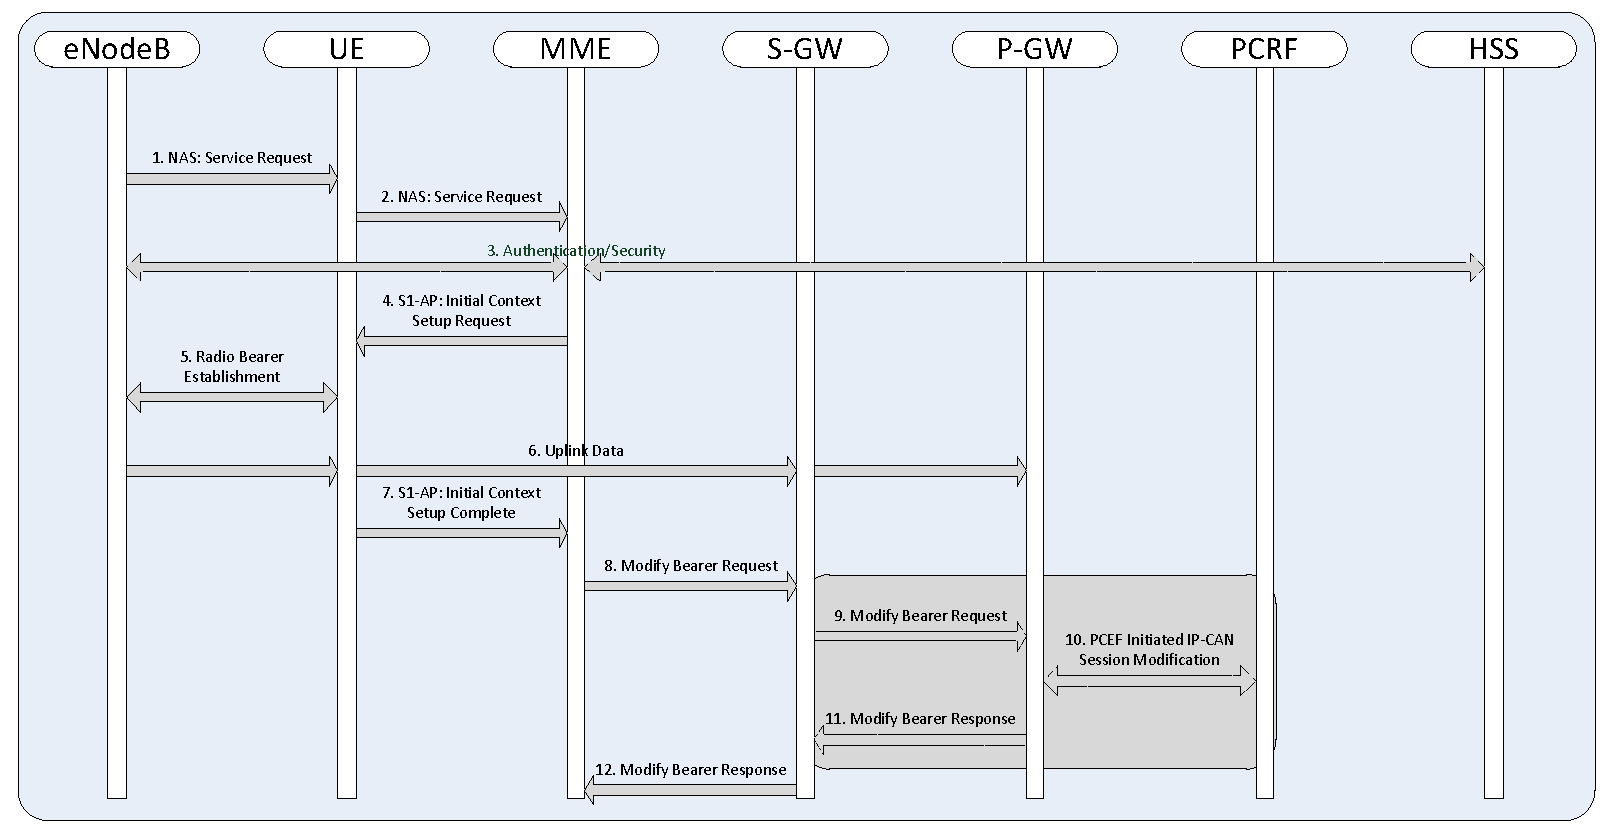
\includegraphics[width=1.0\textwidth]{images/3gpp/UE-service-request.pdf}
 \caption{Beispielnetz}\label{fig:3gpp-ueservicereq}
\end{figure}

Annotations:
1. Encapsulated in RRC message.
2. Forwarded in S1-AP Initial UE Message.
3. Various security procedures.


\section{Information Storage}
per PLMN node, cf. 3GPP TS 23.401 clause 5.7.

\begin{figure}[htbp]
 \centering
 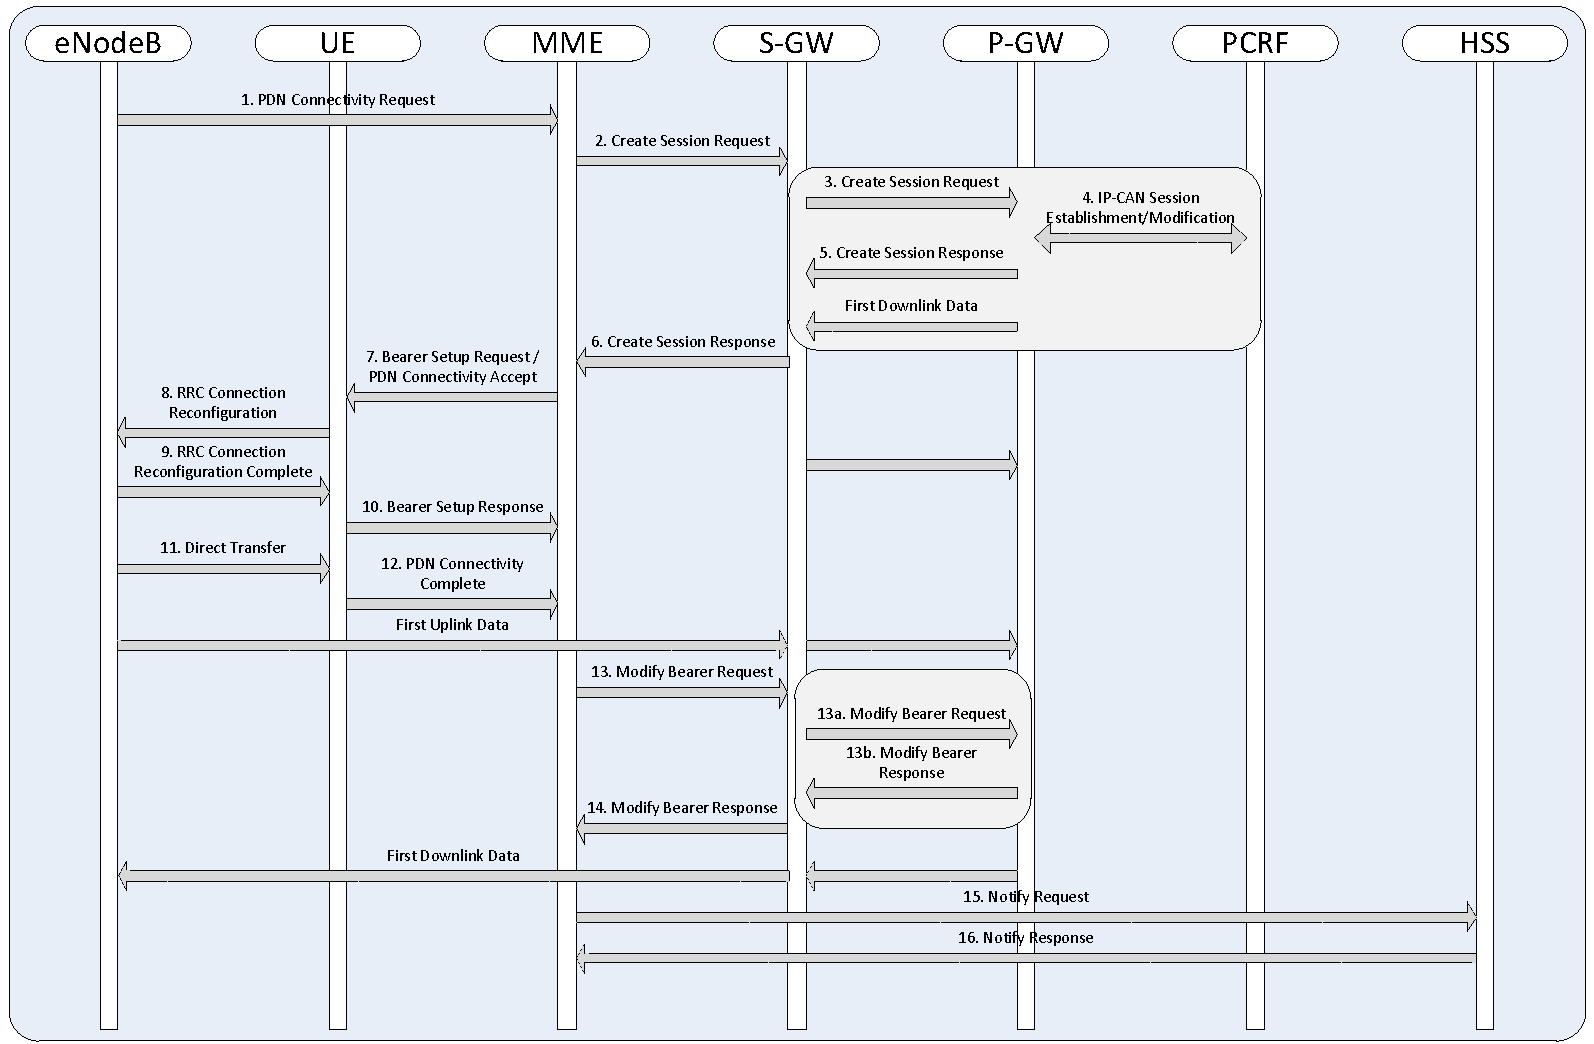
\includegraphics[width=1.0\textwidth]{images/3gpp/UE-requested-PDN-connectivity.pdf}
 \caption{Beispielnetz}\label{fig:3gpp-uepdnreq}
\end{figure}


\section{GTP}
\subsection{GTPv2}



\begin{tabular}{c|c|c|c|c|c|c|c|c|}
\multicolumn{1}{c}{} & \multicolumn{8}{c}{\textbf{Bits}} \\
\cline{2-9} \textbf{Octets} & 8 & 7 & 6 & 5 & 4 & 3 & 2 & 1 \\ 
\cline{2-9} 1 & \multicolumn{3}{c|}{Version}  & P & T & Spare & Spare & Spare \\ 
\cline{2-9} 2 & \multicolumn{8}{c|}{Message Type}  \\ 
\cline{2-9} 3 & \multicolumn{8}{c|}{Message Length (1st Octet)}  \\ 
\cline{2-9} 4 & \multicolumn{8}{c|}{Message Length (2nd Octet)}  \\ 
\cline{2-9} m to & \multicolumn{8}{c|}{\multirow{2}{10cm}{If T flag is set to 1, then TEID shall be placed into octets 5-8. Otherwise, TEID field is not present at all.}} \\ 
 k(m+3) & \multicolumn{8}{c|}{} \\ 
\cline{2-9} n to (n+2) & \multicolumn{8}{c|}{Sequence Number} \\ 
\cline{2-9} (n+3) & \multicolumn{8}{c|}{Spare} \\ 
\cline{2-9} 
\end{tabular} 
\subsection{GTP-C}

\begin{tabular}{c|c|c|c|c|c|c|c|c|}
\multicolumn{1}{c}{} & \multicolumn{8}{c}{\textbf{Bits}} \\
\cline{2-9} \textbf{Octets} & 8 & 7 & 6 & 5 & 4 & 3 & 2 & 1 \\ 
\cline{2-9} 1 & \multicolumn{3}{c|}{Version}  & P & T=1 & Spare & Spare & Spare \\ 
\cline{2-9} 2 & \multicolumn{8}{c|}{Message Type}  \\ 
\cline{2-9} 3 & \multicolumn{8}{c|}{Message Length (1st Octet)}  \\ 
\cline{2-9} 4 & \multicolumn{8}{c|}{Message Length (2nd Octet)}  \\ 
\cline{2-9} 5 & \multicolumn{8}{c|}{Tunnel Endpoint Identifier (1st Octet)} \\ 
\cline{2-9} 6 & \multicolumn{8}{c|}{Tunnel Endpoint Identifier (2nd Octet)} \\ 
\cline{2-9} 7 & \multicolumn{8}{c|}{Tunnel Endpoint Identifier (3rd Octet)} \\ 
\cline{2-9} 8 & \multicolumn{8}{c|}{Tunnel Endpoint Identifier (4th Octet)} \\ 
\cline{2-9} 9 & \multicolumn{8}{c|}{Sequence Number (1st Octet)} \\
\cline{2-9} 10 & \multicolumn{8}{c|}{Sequence Number (2nd Octet)} \\
\cline{2-9} 11 & \multicolumn{8}{c|}{Sequence Number (3rd Octet)} \\
\cline{2-9} 12 & \multicolumn{8}{c|}{Spare} \\
\cline{2-9}
\end{tabular} 

12 Byte GTPv2-C header.

\subsubsection{Create Session Request Message}

Information Elements Table for PDP Context Activation Case only

\begin{longtabu}{|p{2cm}|c|p{1.5cm}|p{8cm}|}
\hline
Information Element 						& IE Type 					& Max Wire Size (Bytes)	& Comment \\ \hline
IMSI 										& IMSI 						& 12					& \\ \hline
MSISDN 										& MSISDN					& 12					& On S11 Interface if provided by HSS; In case of UE requested connectivity if MME has it stored. \\ \hline
MEI Identity 								& MEI 						& 12					& If available at MME. \\ \hline
User Location Information 					& ULI						& 						& E-UTRAN initial attach \&  UE requested connectivity only; included by S-GW if received from MME via S5/S8; included on S4 and S5/S8 for PDP context activation, either CGI, SAI, or RAI. \\ \hline
Serving Network								& Serving Network			& 						& Initial E-UTRAN attach, context activation and UE requested connectivity \\ \hline
RAT Type									& RAT Type					& 5						& \\ \hline
Indication Flags							& Indication				& 6						& Flags: S5/S8 Protocol Type; Dual Address Bearer Flag; Handover Indication; Direct Tunnel Flag; Piggybacking Supported; Change Reporting Support Indication \\ \hline
Sender F-TEID for Control Plane				& F-TEID					& 						& \\ \hline
P-G S5/S8 Address for Control Plane or PMIP	& F-TEID					& 						& On S11/S4 interfaces; 0 if initial attach, context activation or PDN connectivity \\ \hline
Access Point Name							& APN						& 83					& \\ \hline
Selection Mode								& Selection Mode			& 						& Indicate whether subscribed or non-subscribed, chosen by MME, was selected \\ \hline
PDN Type									& PDN Type					& 						& IPv4, IPv6 or IPv4v6. \\ \hline
PDN Address Allocation						& PAA						& 26					& Set to static IP address; else (dynamic) to 0.0.0.0 or IPv6 Prefix Length 0. \\ \hline
Maximum APN Restriction						& APN Restriction			& 						& Set to most stringent restriction of any active bearer. \\ \hline
Aggregate Maximum Bit Rate					& ABMR						& 12					& \\ \hline
Protocol Configuration Options				& PCO						& 254					& Forwarded from UE to P-GW via S-GW via MME. \\ \hline
Bearer Contexts to be created				& Bearer Context			& 						& present multiple times to represent list of bearers \\ \hline
Trace Information							& Trace Information 		& 						& If S-GW / P-GW is activated. \\ \hline
Recovery									& Recovery					& 5						& If peer node contacted for the first time. \\ \hline
MME-FQ-CSID									& FQ-CSID					& 						& Included by MME on S11 \\ \hline
SGW-FQ-CSID									& FQ-CSID					& 						& Included by S-GW on S5/S8 \\ \hline
UE Time Zone								& UE Time Zone 				& 						& Can be included by MME on S11; forwarded to P-GW via S-GW \\ \hline
User CSG Information						& UCI						& 						& If UE accessed via CSG cell or hybrid cell \\ \hline
Charging Characteristics					& Charging Characteristics	&						& \\ \hline
Private Extensions							& Private Extensions		&						& \\ \hline

\end{longtabu}

\subsubsection{Information Elements Wire Format}

\paragraph{IMSI}

\begin{tabular}{c|p{1cm}|p{1cm}|p{1cm}|p{1cm}|p{1cm}|p{1cm}|p{1cm}|p{1cm}|}
\multicolumn{1}{c}{} & \multicolumn{8}{c}{\textbf{Bits}} \\
\cline{2-9} \textbf{Octets} & 8 & 7 & 6 & 5 & 4 & 3 & 2 & 1 \\ 
\cline{2-9} 1 & \multicolumn{8}{c|}{Type = 1 (decimal)} \\ 
\cline{2-9} 2 to 3 & \multicolumn{8}{c|}{Length = n}  \\ 
\cline{2-9} 4 & \multicolumn{4}{c|}{Spare} & \multicolumn{4}{c|}{Instance} \\ 
\cline{2-9} 5 & \multicolumn{4}{c|}{Number digit 2} & \multicolumn{4}{c|}{Number digit 1} \\ 
\cline{2-9} 6 & \multicolumn{4}{c|}{Number digit 4} & \multicolumn{4}{c|}{Number digit 3} \\ 
\cline{2-9} ... & \multicolumn{4}{c|}{...} & \multicolumn{4}{c|}{...} \\ 
\cline{2-9} n+4 & \multicolumn{4}{c|}{Number digit m} & \multicolumn{4}{c|}{Number digit m-1} \\ 
\cline{2-9}
\end{tabular} 

Decimals coded as TBCD; if odd number fill last nibble with 1; max digits is 15.\\
Max IE size 12 Byte.

\paragraph{APN}

\begin{tabular}{c|p{1cm}|p{1cm}|p{1cm}|p{1cm}|p{1cm}|p{1cm}|p{1cm}|p{1cm}|}
\multicolumn{1}{c}{} & \multicolumn{8}{c}{\textbf{Bits}} \\
\cline{2-9} \textbf{Octets} & 8 & 7 & 6 & 5 & 4 & 3 & 2 & 1 \\ 
\cline{2-9} 1 & \multicolumn{8}{c|}{Type = 71 (decimal)} \\ 
\cline{2-9} 2 to 3 & \multicolumn{8}{c|}{Length = n}  \\ 
\cline{2-9} 4 & \multicolumn{4}{c|}{Spare} & \multicolumn{4}{c|}{Instance} \\ 
\cline{2-9} 5 to (n+4) & \multicolumn{8}{c|}{Access Point Name} \\ 
\cline{2-9}
\end{tabular} 

Full APN name including APN Network Identifier and APN Operator Identifier.
Network Identifier: max length 63 bytes.
Operator Identifier: mnc<3digits>.mcc<3digits>.gprs; 16 bytes (18 incl dots).
(Ex: ggsn-cluster-A.provinceB.mnc012.mcc345.gprs)

Max total $4+63+16=83$

\paragraph{AMBR}

\begin{tabular}{c|p{1cm}|p{1cm}|p{1cm}|p{1cm}|p{1cm}|p{1cm}|p{1cm}|p{1cm}|}
\multicolumn{1}{c}{} & \multicolumn{8}{c}{\textbf{Bits}} \\
\cline{2-9} \textbf{Octets} & 8 & 7 & 6 & 5 & 4 & 3 & 2 & 1 \\ 
\cline{2-9} 1 & \multicolumn{8}{c|}{Type = 72 (decimal)} \\ 
\cline{2-9} 2 to 3 & \multicolumn{8}{c|}{Length = n}  \\ 
\cline{2-9} 4 & \multicolumn{4}{c|}{Spare} & \multicolumn{4}{c|}{Instance} \\ 
\cline{2-9} 5 to 8 & \multicolumn{8}{c|}{APN-AMBR for uplink} \\ 
\cline{2-9} 9 to 12 & \multicolumn{8}{c|}{APN-AMBR for downlink} \\ 
\cline{2-9}
\end{tabular} 


Total size 12 bytes.


\paragraph{Recovery}

\begin{tabular}{c|p{1cm}|p{1cm}|p{1cm}|p{1cm}|p{1cm}|p{1cm}|p{1cm}|p{1cm}|}
\multicolumn{1}{c}{} & \multicolumn{8}{c}{\textbf{Bits}} \\
\cline{2-9} \textbf{Octets} & 8 & 7 & 6 & 5 & 4 & 3 & 2 & 1 \\ 
\cline{2-9} 1 & \multicolumn{8}{c|}{Type = 3 (decimal)} \\ 
\cline{2-9} 2 to 3 & \multicolumn{8}{c|}{Length = n}  \\ 
\cline{2-9} 4 & \multicolumn{4}{c|}{Spare} & \multicolumn{4}{c|}{Instance} \\ 
\cline{2-9} 5 to (n+4) & \multicolumn{8}{c|}{Recovery (Restart Counter} \\ 
\cline{2-9}
\end{tabular} 

IN GTPv2 first release IE length is 5 bytes. May be longer in the future.


\paragraph{MEI}

\begin{tabular}{c|p{1cm}|p{1cm}|p{1cm}|p{1cm}|p{1cm}|p{1cm}|p{1cm}|p{1cm}|}
\multicolumn{1}{c}{} & \multicolumn{8}{c}{\textbf{Bits}} \\
\cline{2-9} \textbf{Octets} & 8 & 7 & 6 & 5 & 4 & 3 & 2 & 1 \\ 
\cline{2-9} 1 & \multicolumn{8}{c|}{Type = 75 (decimal)} \\ 
\cline{2-9} 2 to 3 & \multicolumn{8}{c|}{Length = n}  \\ 
\cline{2-9} 4 & \multicolumn{4}{c|}{Spare} & \multicolumn{4}{c|}{Instance} \\ 
\cline{2-9} 5 to (n+4) & \multicolumn{8}{c|}{Mobile Equipment (ME) Identity} \\ 
\cline{2-9}
\end{tabular} 

15 (IMEI) or 16 (IMEISV) BCD digits filled with 1 to full octet. Size is 12 bytes.

\paragraph{MSISDN}

\begin{tabular}{c|p{1cm}|p{1cm}|p{1cm}|p{1cm}|p{1cm}|p{1cm}|p{1cm}|p{1cm}|}
\multicolumn{1}{c}{} & \multicolumn{8}{c}{\textbf{Bits}} \\
\cline{2-9} \textbf{Octets} & 8 & 7 & 6 & 5 & 4 & 3 & 2 & 1 \\ 
\cline{2-9} 1 & \multicolumn{8}{c|}{Type = 76 (decimal)} \\ 
\cline{2-9} 2 to 3 & \multicolumn{8}{c|}{Length = n}  \\ 
\cline{2-9} 4 & \multicolumn{4}{c|}{Spare} & \multicolumn{4}{c|}{Instance} \\ 
\cline{2-9} 5 & \multicolumn{4}{c|}{Number digit 2} & \multicolumn{4}{c|}{Number digit 1} \\ 
\cline{2-9} 6 & \multicolumn{4}{c|}{Number digit 4} & \multicolumn{4}{c|}{Number digit 3} \\ 
\cline{2-9} ... & \multicolumn{4}{c|}{...} & \multicolumn{4}{c|}{...} \\ 
\cline{2-9} n+4 & \multicolumn{4}{c|}{Number digit m} & \multicolumn{4}{c|}{Number digit m-1} \\ 
\cline{2-9}
\end{tabular} 

MSISDN limited to 15 digits. Max total size 12 bytes.


\paragraph{Indication}
\centering
\begin{tabular}{c|p{1cm}|p{1cm}|p{1cm}|p{1cm}|p{1cm}|p{1cm}|p{1cm}|p{1cm}|}
\multicolumn{1}{c}{} & \multicolumn{8}{c}{\textbf{Bits}} \\
\cline{2-9} \textbf{Octets} & 8 & 7 & 6 & 5 & 4 & 3 & 2 & 1 \\ 
\cline{2-9} 1 & \multicolumn{8}{c|}{Type = 77 (decimal)} \\ 
\cline{2-9} 2 to 3 & \multicolumn{8}{c|}{Length = n}  \\ 
\cline{2-9} 4 & \multicolumn{4}{c|}{Spare} & \multicolumn{4}{c|}{Instance} \\ 
\cline{2-9} 5 & DAF & DTF & HI & DFI & OI & ISRSI & ISRAI & SGWCI \\ 
\cline{2-9} 6 & Spare & UIMSI & CFSI & CRSI & P & PT & SI & MSV \\ 
\cline{2-9} 7 to (n+4) & \multicolumn{8}{c|}{These octet(s) is/are present only if explicitly specified} \\ 
\cline{2-9}
\end{tabular} 

Size is 7 bytes.

\paragraph{PCO}
\centering
\begin{tabular}{c|p{1cm}|p{1cm}|p{1cm}|p{1cm}|p{1cm}|p{1cm}|p{1cm}|p{1cm}|}
\multicolumn{1}{c}{} & \multicolumn{8}{c}{\textbf{Bits}} \\
\cline{2-9} \textbf{Octets} & 8 & 7 & 6 & 5 & 4 & 3 & 2 & 1 \\ 
\cline{2-9} 1 & \multicolumn{8}{c|}{Type = 78 (decimal)} \\ 
\cline{2-9} 2 to 3 & \multicolumn{8}{c|}{Length = n}  \\ 
\cline{2-9} 4 & \multicolumn{4}{c|}{Spare} & \multicolumn{4}{c|}{Instance} \\ 
\cline{2-9} 5 to (n+4) & \multicolumn{8}{c|}{Protocol Configuration Options} \\
\cline{2-9}
\end{tabular} 

Minimum length 4+3-3, maximum length 4+253-3; average?


\paragraph{PAA}
\centering

\begin{tabular}{c|p{1cm}|p{1cm}|p{1cm}|p{1cm}|p{1cm}|p{1cm}|p{1cm}|p{1cm}|}
\multicolumn{1}{c}{} & \multicolumn{8}{c}{\textbf{Bits}} \\
\cline{2-9} \textbf{Octets} & 8 & 7 & 6 & 5 & 4 & 3 & 2 & 1 \\ 
\cline{2-9} 1 & \multicolumn{8}{c|}{Type = 79 (decimal)} \\ 
\cline{2-9} 2 to 3 & \multicolumn{8}{c|}{Length = n}  \\ 
\cline{2-9} 4 & \multicolumn{4}{c|}{Spare} & \multicolumn{4}{c|}{Instance} \\ 
\cline{2-9} 5 & \multicolumn{5}{c|}{Spare} & \multicolumn{3}{c|}{PDN Type} \\
\cline{2-9} 6 to (n+4) & \multicolumn{8}{c|}{PDN Adress and Prefix} \\
\cline{2-9}
\end{tabular} 

Either 9 (IPv4), 22 (IPv6), or 26 (IPv4v6).


\paragraph{RAT Type}
\centering
\begin{tabular}{c|p{1cm}|p{1cm}|p{1cm}|p{1cm}|p{1cm}|p{1cm}|p{1cm}|p{1cm}|}
\multicolumn{1}{c}{} & \multicolumn{8}{c}{\textbf{Bits}} \\
\cline{2-9} \textbf{Octets} & 8 & 7 & 6 & 5 & 4 & 3 & 2 & 1 \\ 
\cline{2-9} 1 & \multicolumn{8}{c|}{Type = 82 (decimal)} \\ 
\cline{2-9} 2 to 3 & \multicolumn{8}{c|}{Length = n}  \\ 
\cline{2-9} 4 & \multicolumn{4}{c|}{Spare} & \multicolumn{4}{c|}{Instance} \\ 
\cline{2-9} 5 & \multicolumn{8}{c|}{RAT Type} \\
\cline{2-9} 6 to (n+4) & \multicolumn{8}{c|}{These octet(s) is/are present only if explicitly specified} \\
\cline{2-9}
\end{tabular} 

Maximum length 5 to ?.

\paragraph{Serving Network}

\centering
\begin{tabular}{c|p{1cm}|p{1cm}|p{1cm}|p{1cm}|p{1cm}|p{1cm}|p{1cm}|p{1cm}|}
\multicolumn{1}{c}{} & \multicolumn{8}{c}{\textbf{Bits}} \\
\cline{2-9} \textbf{Octets} & 8 & 7 & 6 & 5 & 4 & 3 & 2 & 1 \\ 
\cline{2-9} 1 & \multicolumn{8}{c|}{Type = 83 (decimal)} \\ 
\cline{2-9} 2 to 3 & \multicolumn{8}{c|}{Length = n}  \\ 
\cline{2-9} 4 & \multicolumn{4}{c|}{Spare} & \multicolumn{4}{c|}{Instance} \\ 
\cline{2-9} 5 & \multicolumn{4}{c|}{MCC digit 2} & \multicolumn{4}{c|}{MCC digit 1} \\ 
\cline{2-9} 6 & \multicolumn{4}{c|}{MNC digit 3} & \multicolumn{4}{c|}{MCC digit 3} \\ 
\cline{2-9} 7 & \multicolumn{4}{c|}{MNC digit 2} & \multicolumn{4}{c|}{MNC digit 1} \\ 
\cline{2-9} 8 to (n+4) & \multicolumn{8}{c|}{These octet(s) is/are present only if explicitly specified} \\
\cline{2-9}
\end{tabular} 

Maximum length 7 to ?.


\paragraph{User Location Information}

\centering
\begin{tabular}{c|p{1cm}|p{1cm}|p{1cm}|p{1cm}|p{1cm}|p{1cm}|p{1cm}|p{1cm}|}
\multicolumn{1}{c}{} & \multicolumn{8}{c}{\textbf{Bits}} \\
\cline{2-9} \textbf{Octets} & 8 & 7 & 6 & 5 & 4 & 3 & 2 & 1 \\ 
\cline{2-9} 1 & \multicolumn{8}{c|}{Type = 86 (decimal)} \\ 
\cline{2-9} 2 to 3 & \multicolumn{8}{c|}{Length = n}  \\ 
\cline{2-9} 4 & \multicolumn{4}{c|}{Spare} & \multicolumn{4}{c|}{Instance} \\ 
\cline{2-9} 5 & \multicolumn{3}{c|}{Spare} & ECGI & TAI & RAI & SAI & CGI \\ 
\cline{2-9} a to a+6 & \multicolumn{8}{c|}{CGI} \\ 
\cline{2-9} 7 & \multicolumn{8}{c|}{SAI} \\ 
\cline{2-9} 7 & \multicolumn{8}{c|}{RAI} \\ 
\cline{2-9} 7 & \multicolumn{8}{c|}{TAI} \\ 
\cline{2-9} 7 & \multicolumn{8}{c|}{ECGI} \\ 
\cline{2-9} 8 to (n+4) & \multicolumn{8}{c|}{These octet(s) is/are present only if explicitly specified} \\
\cline{2-9}
\end{tabular} 


\subsection{GTP-U}
